% Encoding: UTF-8 (UNIX line breaks)
% Author: Ivan Ramos Pagnossin

\documentclass{article}
	%\usepackage[latin1]{inputenc}
	\usepackage[utf8]{inputenc}
	\usepackage[T1]{fontenc}
	\usepackage[english,brazil]{babel}
	\usepackage{sbc-template}
	%\usepackage{paralist}
	\usepackage{url}
	\usepackage{amsmath}
	\usepackage{graphicx}

\title{Sistema multi-agentes em atividades colaborativas sobre empirismo nas ciências}
\author{Ivan R. Pagnossin\inst{1}, Arthur Tofani\inst{1}, Gil da C. Marques\inst{1}}

\address{
	Centro de Ensino e Pesquisa Aplicada --- Instituto de Física da Universidade de São Paulo\\
	Rua do Matão, travessa R nº 187, Edifício Van de Graaf\\
	Cidade Universitária, CEP 05508-090, São Paulo, Brasil
\email{irpagnossin@usp.br, arthur.tofani@usp.br, marques@if.usp.br}
}

\begin{document}

\maketitle

\selectlanguage{english}
\begin{abstract}
In this work we present a collaborative learning object (LO) based on multi-agent systems,
developed with the purpose of emphasize the empiricism as the basis of science (through the scientific method).
We also present a proposal of application for this LO in Learning Management Systems,
and some preliminary qualitative results of its application in the undergraduation science course of the agreement USP/UNIVESP.

\begin{description}
\item[Learning object:] \url{cepa.if.usp.br/ivan/AI-0109}
\item[Screenshot:] \url{cepa.if.usp.br/ivan/AI-0109/AI-0109.jpg}
\item[License:] Creative Commons CC BY-NC-SA 3.0
\end{description}
\end{abstract}

\selectlanguage{brazil}
\begin{abstract}
Neste trabalho nós apresentamos um objeto de aprendizagem (OA) colaborativo baseado em sistemas multi-agentes (SMA),
desenvolvido com o propósito de evidenciar o empirismo como base das ciências (através do método científico).
Apresentamos também a proposta de aplicação deste OA em Ambientes Virtuais de Aprendizagem e os primeiros resultados qualitativos
observados, decorrentes de sua aplicação no curso de Eletromagnetismo (PLC0012 do sistema Júpiter) da graduação em
Licenciatura em Ciências do convênio USP/UNIVESP (Universidade Virtual do Estado de São Paulo).
\end{abstract}

\section{Introdução}

O termo empirismo refere-se a toda doutrina para o qual o conhecimento só pode
ser alcançado mediante a experiência sensorial (dicionário Aulete). Ele baseia-se
na capacidade de observação da natureza: percepção dos elementos que a compõem,
observação de fenômenos e identificação das relações de causa e consequência. Esta
ideia, proposta por John Locke no séc. XVI, ainda hoje é base do método científico,
mas é comumente transmitida aos alunos das áreas das ciências de forma indireta,
usualmente agregada a práticas de laboratório em diversas disciplinas, como Física,
Química e Biologia. Seu estudo isolado dos contextos já familiares aos alunos, por outro
lado, é potencialmente desestimulante e de difícil absorção. Além disso, a indissociação
deste conceito às práticas de laboratório tem apresentado efeitos colaterais sutis,
como a usual incompreensão de que o termo \emph{carga elétrica}, por exemplo, refere-se
apenas a uma atribuição convenientemente introduzida para explicar os fenômenos do
eletromagnetismo.

\section{A proposta do objeto de aprendizagem}

Sua necessidade apareceu na proposta do curso de Eletromagnetismo do curso de Lic.
em Ciências do convênio USP-UNIVESP, quando o Prof. Dr. Gil da Costa Marques,
autor do curso, propôs conduzir a didática do curso através de uma outra abordagem,
tendo a carga como sendo o atributo da matéria de maior relevância (e não o campo
eletromagnético). A carga, porém, é um atributo meramente teórico oriundo unicamente
da observação do comportamento da matéria, obtido portanto por meio do empirismo –
e seria portanto fundamental cultivar no aluno tal entendimento.

Foi neste contexto que surgiu a proposta do OA em questão: permitir ao aluno
perceber empiricamente atributos de entes físicos. Para isso, criamos o que chamamos
de “mundo virtual”, onde elementos (agentes, no contexto da computação) interagem
entre si através de poucas leis simples. Este trabalho sintetiza-se, portanto, pela intenção
de se criar uma abordagem ao empirismo de forma abstrata, que não apresente relação
direta com os motivos aos quais este conceito aparece sempre ligado.

A intenção inicial foi de criar um sistema com uma complexidade tal que seu
comportamento, à primeira vista, parecesse caótico, mas que com a observação
sistematizada fosse possível extrair dele (parte 1) os atributos que caracterizam os
elementos que compõem este mundo, (2) as leis que o regem e (3) uma modelagem
matemática desses atributos e leis, dando assim aos alunos a oportunidade de não
apenas experimentar o empirismo por sua essência, mas também o método científico e a
modelagem matemática desses “fenômenos”. Este software, no entanto, é apenas uma
das partes envolvidas na atividade proposta. Além dele, criamos um fórum de
discussões intitulado “Comunidade científica”, cujo propósito é promover a discussão
entre os alunos (então cientistas neste cenário), simulando de fato a comunidade
científica de uma área qualquer. Outra componente indispensável da atividade é os
tutores do curso, que foram orientados por nós quanto à mediação dessas discussões.

\section{Sistema multi-agentes}

O conceito de sistemas multi-agentes é inspirado na ideia de agentes independentes
coexistentes dentro de um mesmo ambiente. Cada agente é um subprograma com
certa autonomia dentro daquele ambiente, e é composto de rotinas de caráter sensorial,
por onde o mesmo é capaz de perceber o ambiente (incluindo outros agentes e a si
mesmo), rotinas de raciocínio, nas quais o agente toma decisões baseadas nos estímulos
recebidos pelos sensores, e rotinas de ação, onde de acordo com suas heurísticas de
raciocínio, o agente pode produzir informação dentro do sistema onde está inserido.

Pela definição de \cite{reis-2002}, ``um agente é um sistema computacional, situado
num dado ambiente, que tem a percepção desse ambiente através de sensores, tem
capacidade de decisão, age de forma autônoma nesse ambiente através de atuadores, e
possui capacidades de comunicação de alto nível com outros agentes e/ou humanos, de
forma a desempenhar uma dada função para a qual foi projetado''. O diagrama
apresentado por \cite{Thomaz-2011}, baseado na generalização de diversos outros trabalhos,
ilustra a arquitetura de um agente da maneira como foi utilizada para este trabalho:

\begin{figure}
	\centering
	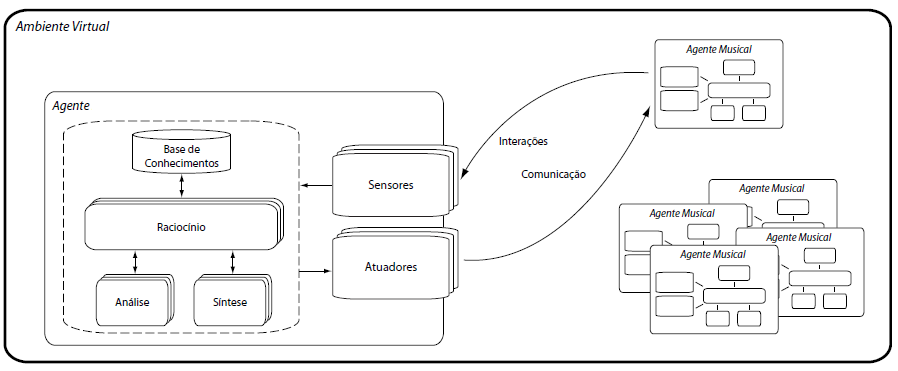
\includegraphics[width=\textwidth]{figures/agent}
	\caption{Diagrama esquemático de um agente}
	\label{fig:mas}
\end{figure}

A arquitetura de sistemas multi-agentes tem se mostrado bastante poderosa,
sobretudo por adequar-se a técnicas de processamento paralelo e computação em nuvem.
No entanto, sua grande contribuição está em produzir resultados dificilmente
alcançados em sistemas monolíticos, onde o controle de todos os elementos é
centralizado. O processamento dos raciocínios e ações se dá por escalonamento em
turnos, uma vez que a aplicação trabalha com single-thread, conforme a proposta de
\cite{behrens-2010} para sistemas multi-agentes em ambientes de jogos virtuais.
De acordo com a proposta deste objeto de aprendizagem, o aluno deve ser capaz
de observar as interações correntes entre elementos em um mundo hipotético que lhe
será apresentado. A decisão de desenvolver este dispositivo baseado na arquitetura de
sistemas multi-agentes foi baseada na versatilidade na criação dos sensores e atuadores
destes agentes, permitindo que se buscasse uma configuração de agentes que atendesse
adequadamente aos objetivos pedagógicos. Além disso, em um primeiro momento
deseja-se criar uma configuração abstrata que não tenha relação direta com fenômenos
naturais observáveis pelos alunos; uma segunda versão, porém, pode vir a ser uma
variação do mesmo objeto de aprendizagem, que utilizando a mesma estrutura poderá
vir a ilustrar algum fenômeno real (atração e repulsão de cargas eletromagnéticas,
combinações genéticas, a relação entre pressão, temperatura e volume, etc).

\section{Planejamento do ``mundo virtual''}

O ambiente deste sistema foi criado no formato de um tabuleiro, supondo que as peças
só podem andar em quatro sentidos (cima, baixo, esquerda, direita), sobre as linhas
deste tabuleiro, com um modelo de agente que atende às seguintes características
físicas: (1) forma poligonal, podendo assumir uma entre três formas possíveis:
triângulo, quadrado ou pentágono, (2) cor , podendo assumir as cores verde, azul e roxa,
(3) rotação no próprio eixo, que pode ou não ocorrer no agente.

Os raciocínios dos agentes são relacionados à sua movimentação apenas.
Axiomaticamente, as peças não podem ocupar o mesmo espaço no tabuleiro. O
raciocínio geral para todos os agentes diz que eles devem buscar manter inerte a direção
e o sentido do seu movimento, a menos que algo obstrua seu caminho, situação na qual
deverá buscar uma nova direção livre para continuar caminhando, de acordo com uma
ordem de “preferências”, determinada pela característica de cor do agente neste
momento, conforme a tabela ~\ref{tab:cor-vs-movimentacao}.

\footnotesize

\begin{table}
\begin{center}
	\begin{tabular}{ll}		
		Cor do agente & Preferências de movimentação \\
		\hline \hline
		Azul          & Direita, esquerda \\
		Verde         & Cima, baixo \\
		Roxo          & Direita, esquerda, cima, baixo
	\end{tabular}
	\caption{Movimentação dos agentes segundo suas cores}
	\label{tab:cor-vs-movimentacao}
\end{center}
\end{table}

\normalsize
No caso da colisão entre dois agentes, suas características são modificadas de
acordo com o seguinte algoritmo:

Sejam $a_1$ e $a_2$ os agentes em colisão. Atribui-se os seguintes valores para as cores $c_1$ e $c_2$: Azul = 1; Verde = 2; Roxo = 3;
Atribui-se os valores para as formas $f_1$ e $f_2$: Quadrado = 1; Triangulo = 2; Pentágono = 3;

\begin{gather}
c_1 = c_2 + c_1 + 1 \mod 3 \qquad\text{e}\qquad c_2 = c_1 c_2 + 1 \mod 3;\\
f_1 = f_2 + f_1 + 1 \mod 3 \qquad\text{e}\qquad f_2 = f_1 f_2 + 1 \mod 3;\\
g_1 = g_2 \qquad\text{e}\qquad g_2 = g_1
\end{gather}

Por exemplo, o agente $a_1$ (Quadrado Azul, girando) colide com $a_2$ (Pentágono Verde, parado),
as novas características de cada agente são $a_1$: triângulo verde, parado;
$a_2$: Quadrado roxo, girando. % TODO: melhorar esse exemplo

\section{Aplicação do OA}

O objeto de aprendizagem foi apresentado aos alunos através do LMS (\emph{Learning
Management System}) Moodle (\url{licenciaturaciencias.usp.br}) como parte das atividades das três primeiras semanas do curso de Eletromagnetismo. 

A atividade consiste em o aluno observar o comportamento dos elementos presentes no mundo virtual e tentar descrever, no fórum associado à atividade, 
o que ele observa. Clicando sobre os agentes, o aluno pode movê-los e soltá-los livremente no cenário. Na lateral direita do mundo virtual há um espaço 
definido como \emph{laboratório}, onde o aluno pode isolar agentes para verificar seu comportamento. Colaborativamente, os alunos discutem no fórum
as observações feitas, cabendo aos tutores orientar e organizar o conhecimento construído, buscando que os alunos extraiam de suas observações 
a proposição de um modelo científico capaz de traduzir os fenômenos ocorrentes naquele sistema. Ademais, o tutor deve conduzir os alunos no 
refinamento deste modelo, na intenção de que o aluno, na medida do possível, decifre as regras de produção daquele comportamento. 


\section{Resultados}

Neste momento (26.10.2011) o objeto de aprendizagem em questão ainda está
sendo aplicado (terceira semana), de modo que ainda não há resultados conclusivos.
Ainda assim pudemos observar alguns fenômenos interessantes, dos quais destacamos
dois (os demais serão apresentados após a conclusão da aplicação do OA em revistas da
área de educação):

\begin{itemize}
\item A maioria dos alunos procurou associar os fenômenos do mundo virtual ao
mundo real, por mais que fossem advertidos quanto à inexistência dessa
associação. Isto pode evidenciar a tese proposta inicialmente, de que existem
efeitos colaterais ao ensino tradicional do método científico, nos laboratórios.
Mas há outra explicação: a atividade foi apresentada simultaneamente aos
conteúdos regulares do curso de Eletromagnetismo, o que pode ter induzido essa
associação.
\item Observamos uma melhora progressiva na organização dos experimentos e na
apresentação do conheciento adquirido, através do fórum. É uma forte evidência
da contribuição do objeto de aprendizagem para o raciocínio científico do aluno,
mas também requer mais análises.
\end{itemize}

\section{Conclusões e perspectivas}

Os resultados parciais da aplicação desse sistema multi-agentes nesta atividade
colaborativa indica ter sido esta uma experiência de sucesso, tanto do ponto de vista
técnico, pois trouxe ganhos de conhecimento para a equipe de programação, como
pedagógico, pois há evidências de contribuição positiva para o aprendizado do aluno.
Entretanto, este é um trabalho em progresso, cujos resultados ainda estão por
vir. Apesar disso, algumas modificações são evidentes: no que concerne o software,
algumas melhorias de experiência do usuário são necessárias, como a redução
do “laboratório” (área do software para a qual o aluno pode fazer experimentos com
os elementos do mundo virtual, de maneira controlada, como num laboratório de fato).
Isto é necessário pois, como está, é difícil fazer colidir os elementos que compõem o
mundo virtual e, por consequência, observar de maneira controlada as leis que o regem.
Mas a alteração mais significativa, que dará origem a uma versão paralela a esta, é a
introdução de leis não-determinísticas. Com isso teremos um objeto de aprendizagem
similar, que poderá ser utilizado na introdução de um curso de Mecânica Quântica.
Há também modificações na metodologia da análise dos resultados dos alunos, mas
deixaremos isto para um meio de divulgação mais apropriado.

\bibliographystyle{sbc}
\bibliography{computation}

\end{document}
